%auto-ignore
% TODO: Fix stuff here
\section{Introduction}

There are currently two main solutions for utilizing NLP tasks with no context provided: 

\begin{enumerate}[leftmargin=1em]
    \item Large Pre-Trained Text-Generation and Text2Text-Generation Model \label{CurrSolOne}
        \begin{itemize}[leftmargin=1em]
            \begin{figure}
                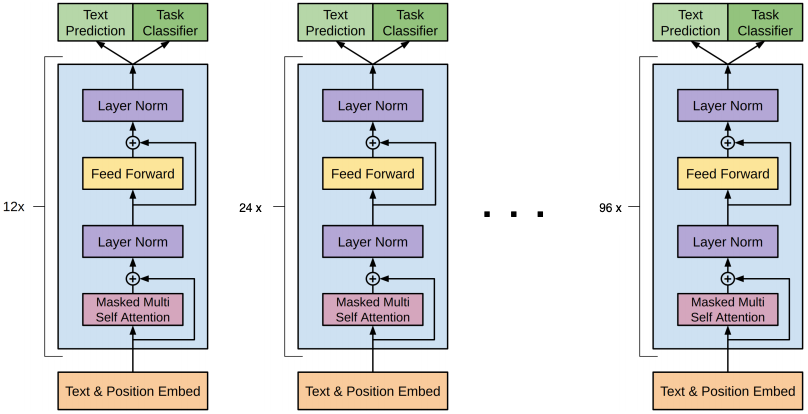
\includegraphics[width=1.0\columnwidth]{gpt3architecture.png}
                \caption{This is an illustration of the architecture of GPT-2 and GPT-3, a popular Text-Generation model \cite{gpt3-overview, the-gpt-3-architecture-on-a-napkin}.}
                \label{fig:CurrSolOneImg}
                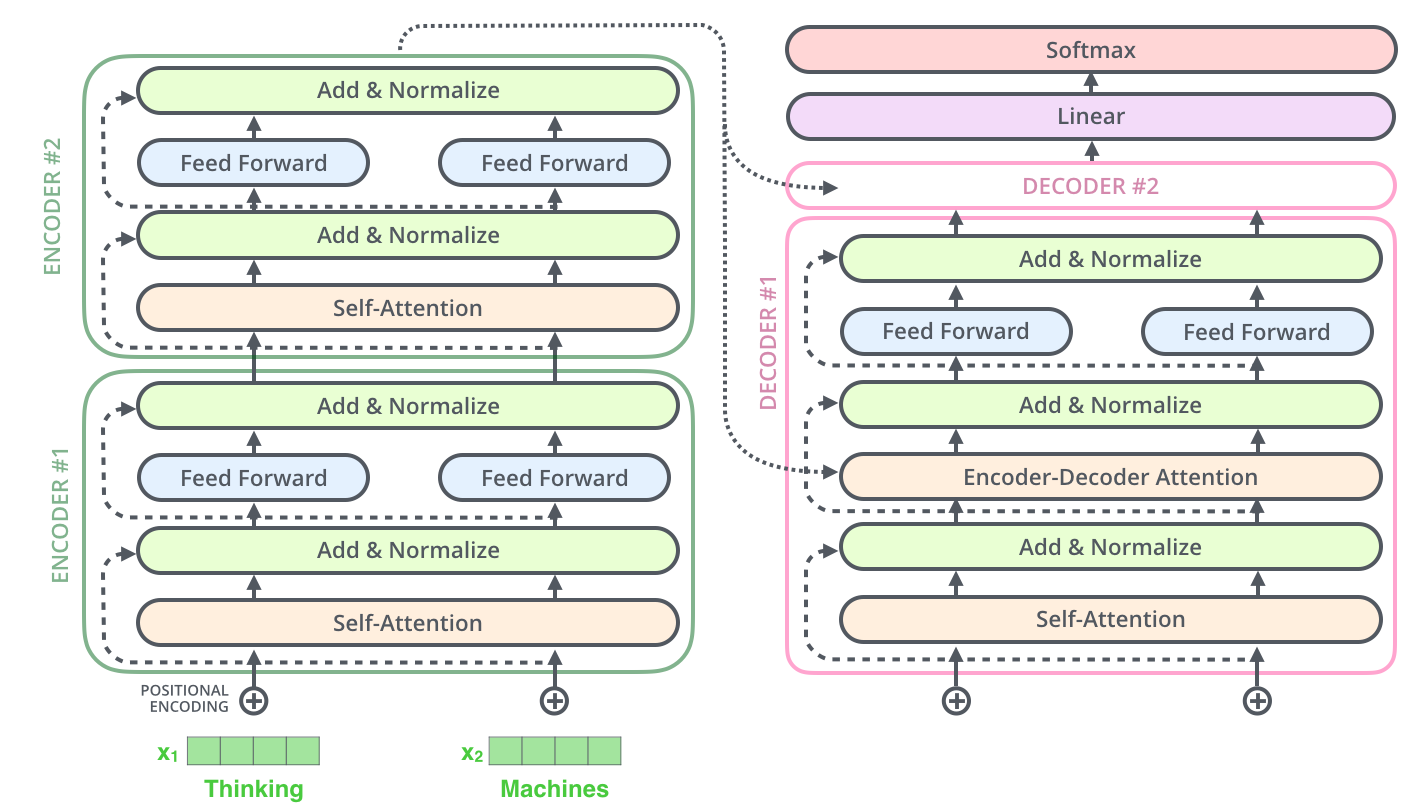
\includegraphics[width=1.0\columnwidth]{t5architecture.png}
                \caption{This is an illustration of the architecture of T5, a popular Text2Text-Generation model \cite{alammar}.}
                \label{fig:CurrSolOneSecondImg}
            \end{figure}
            \item Pre-trained Text-generation models, like GPT-NeoX, GPT-3, and etc. \cite{gpt-neox-20b,gpt-neox-library,DBLP:journals/corr/abs-2005-14165} can be trained for open-domain question-answering closed-book language model tasks (ODQA LM) \cite{weng2020odqa}. When used in ODQA tasks, they achieve SOTA results in such tasks, have high accuracy and are fast but are much larger in size than open-book (context-needing) language models.
            \item Additionally Pre-trained Text2Text-generation models, like T5 \cite{https://doi.org/10.48550/arxiv.1910.10683} that have open-domain question-answering closed-book (no context) language models (ODQA LM) capabilities \cite{weng2020odqa}. These closed-book QDQA LMs are comparatively state-of-the-art performance in many no-context NLP tasks, mainly question-answering. Text2Text-generation models for such no-context NLP tasks are usually large, slow, and have a low accuracy \cite{DBLP:journals/corr/abs-2002-08910}.
            \item Example: T5 \cite{https://doi.org/10.48550/arxiv.1910.10683}
            \item Illustration of how ODQA LM work: \ref{fig:CurrSolOneImg}
        \end{itemize}
    \item Large Knowledge Database with a Contex-Needing Language Model \label{CurrSolTwo}
        \begin{itemize}[leftmargin=1em]
            \begin{figure}
                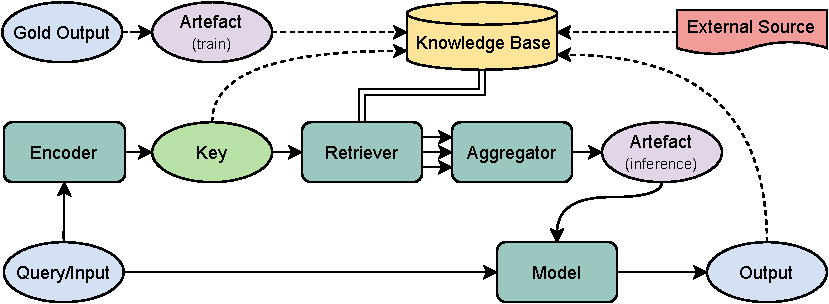
\includegraphics[width=1.0\columnwidth]{artefacts_diagram.pdf}
                \caption{This is an illustration of how LMs with a knowledge base and artifact retriver work \cite{https://doi.org/10.48550/arxiv.2201.09651}.}
                \label{fig:CurrSolTwoImg}
            \end{figure}
            \item Large Knowledge base with an pre-trained open-book LM and retriever, provides an comparatively higher performance, accuracy and the model itself is small. These models however require --- usually --- a large knowledge base which makes the overall solution large, but still fast and with more accuracy on the field the knowledge base specalizes in.
            \item Example: LinkBERT \cite{https://doi.org/10.48550/arxiv.2203.15827} with an artifact retriver \cite{https://doi.org/10.48550/arxiv.2201.09651} with a knowledge base such as DBpedia or WikiData \cite{10.5555/1785162.1785216, 10.1145/2629489}
            \item Illustration of how LMs with a knowledge base and artifact retriver work: \ref{fig:CurrSolTwoImg}
        \end{itemize}
\end{enumerate}

Solution \ref{CurrSolOne} and \ref{CurrSolTwo} achieve the same end goal of NLP tasks without context via two different methods; these current solutions restrict NLP tasks and accuracy without context, especially for more open-domain tasks. The major limitation in this case would be accuracy, efficency and size of models and their knowledge base which then limit the use cases of closed-book open-domain NLP tasks.

In this paper, I propose \inlp, an direct improvement to solution \ref{CurrSolOne} which allows NLP models to not require a large knowledge base (altough you can configure Internet-NLP to utilize a knowledge base) that incoproates the internet's vast knowledge along utilizing data in hyperlinks in webpages \cite{https://doi.org/10.48550/arxiv.2203.15827} to create a more resource-filled data for our existing or future context-needing pre-trained model to use for NLP tasks. Internet-NLP encompasses pre-trained NLP and NLI models, along with its web-data-scraper creates an small temporary on-basis data and a cache for NLP tasks to be performed without given context.

Utilizing the vast data on the internet, graph of documents as corpus \cite{https://doi.org/10.48550/arxiv.2203.15827} allows us to enable to reduce our solution size, increase efficency and increase accuracy. Additionally unlike usage of static data, Internet-NLP utilizes the dynamic, and frequent updating data of the internet which enables us to utilize any type of NLP model along with NLI models to allow us to follow a sequence of control flow to get the context for context-needing models. This approach utilizes a combination of data-collection \cite{inbook} for NLPs with context-needing open-domain NLP to gain more accurate results in most no-context NLP tasks.

Additionally Internet-NLP's Text2Text-generation search query model: T5 \cite{https://doi.org/10.48550/arxiv.1910.10683} and LSTM noun remembrance using parts of speech tagging \cite{Chiche2022} on ALotClosedBookQA with it improving search queries based on the difference on answer recieved and the answer from datasets, using parts of speech tagging on answers \cite{Chiche2022}.
